\chapter{PC aplikace}
Pro účely testeru byla vyvinuta PC aplikace založená na programovacím jazyku python. Tato aplikace umožňuje
nejen komunikovat s testerem a provádět měření, ale také převádět vstupní CAD, CAM, gerber a různé textové konfigurační
soubory do vhodného formátu pro účely testeru.\\




\section{Principy funkce PC aplikace}
Obrázek \ref{fig: PCAPP top level diagram} uvádí velmi zjednodušený a neúplný náhled na strukturu PC aplikace.
PC aplikace je postavena na platformě "TEST API", která je vyvíjena autorem diplomové práce. Platforma je poměrně obsáhlá
a její popis by přesáhl rámec této práce. Z tohoto důvodu bude popsána pouze část platformy, která je pro diplomovou práci nejdůležitější.\\

Aplikace je rozdělena do několika vrstev, každá z vrstev by měla plnit svoji specifickou úlohu a být jakýmsi nezávislým blokem.
PC aplikace se snaží toto "pravidlo" dodržovat nicméně ne všechny bloky jsou kompletně nezávislé.
Použité názvy vrstev nevychází ze žádného standartu jako např. ISO/OSI apod.\\

\begin{figure}[ht!]
    \centering
    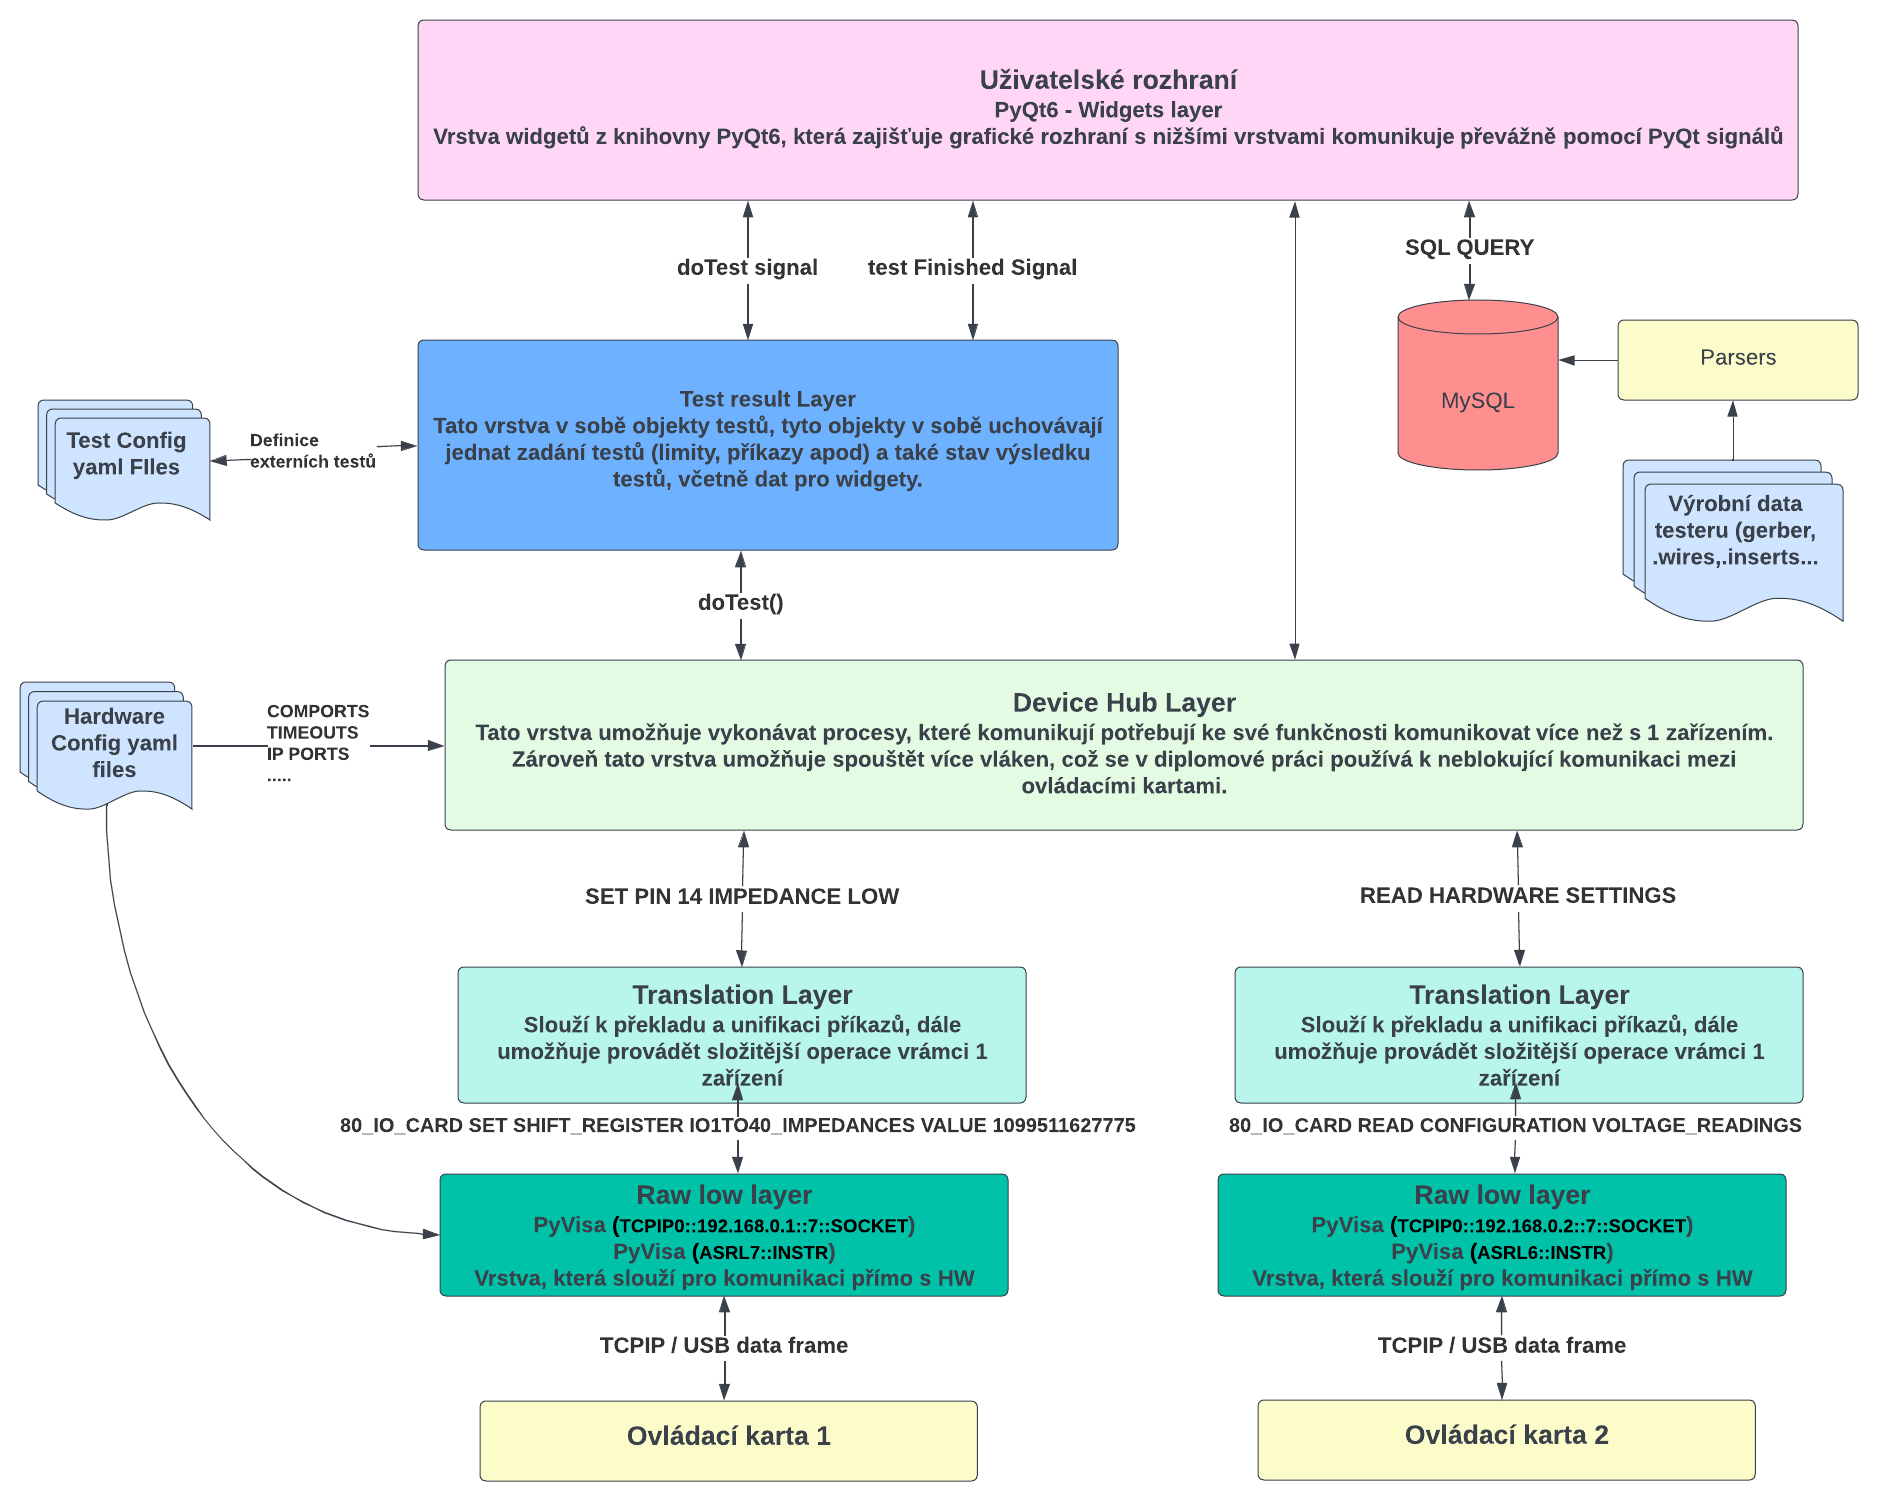
\includegraphics[width = 0.9\textwidth]{obrazky/PC_app_diagram.png}
    \caption{PC aplikace - top level diagram}
    \label{fig: PCAPP top level diagram}
\end{figure}


\section{PC aplikace - Raw low layer}
Nejnižší vrstvou je tzv. Raw low layer. Tato vrstva složí přímo ke komunikaci se zařízením. Převádí tak příkazy z kapitoly 4 do TCP/IP popř. USB rámců.
V případě diplomové práce tuto vrstvu pro ovládací karty zajišťuje knihovna pyVisa, která je založena na knihovně VISA od firmy National Instruments.
Tato knihovna umožňuje pohodlně komunikovat se zařízením přes různé fyzické vrstvy (TCP/IP, USB, RS232, GPIB) a to pomocí jednotného API.\\


\section{PC aplikace - Ttranslation Layer}
Druhou nejnižší vrstvou je tzv. Translation Layer (Překládací vrstva). Úkolem této vrstvy by mělo být poskytnout sofistikovanější funkce, které se skládají z více příkazů,
kterou nabízí komunikační protokol ovládaného zařízení. Zároveň by tato vrstva měla co nejvíce sjednocovat příkazy pro přístroje stejného druhu od různých výrobců.
Tato funkce je však pro diplomovou práci zanedbatelná, protože všechny ovládací karty používají stejný komunikační protokol.\\

Jako příklad funkce této vrstvy uveďmě příkaz pro nastavení výstupní impedance pinu č.14 do nízké impedance, přičemž ostatní piny mají zůstat nezměněny.
Vyšší vrstvy předají příkaz v podobě SET PIN 14 IMPEDANCE LOW. Překládací vrstva nejprve zjistí aktuální hodnotu registru, který určuje impedance jednotlivých pinů.
Dále v závislosti na endianitě pozmění hodnotu registru a odešle příkaz, který nastaví novou hodnotu registru pomocí příkazu
80\_IO\_CAR SET SHIFT\_REGISTER IO1TO40\_IMPEDANCES VALUE "nová hodnota".\\


\section{PC aplikace - Device Hub Layer}
Device Hub Layer má za úkol vykonávat příkazy, které ke své funkcni potřebují více než pouze jedno zařízení.
Typickým případem by bylo nastavení výstupního napětí napájecího zdroje a následné ověření napětí multimetrem.
V diplomové práci byla tato vrstva např. využita k automatizovanému měření průběhů v kapitole 4.\\

Druhým důležitým úkolem této vrstvy je rozřazovat požadované testy do vláken programu a předcházet tak zamrzání.
Z tohoto důvody by veškerá komunikace od vyšších vrstev měla probíhat přes tuto vrstvu.
Tato funkcionalita se hodí pro diplomovou práci, protože umožňuje zasílat příkazy do několika ovládacích karet zároveň a
urychlit tak měření.


\section{PC aplikace - Test Result Layer}
Test Result layer je více než vrstvou spíše objektem.
Není tak striktně ohraničený a z historických důvodů má přesah do některých z nejnižších vrstev.
Do tohoto objektu jsou ukládány výsledky jednotlivých testů (příkazů) a zároveň jsou tyto výsledky vyhodnocovány podle
určitých kritérií.
Test Result Layer se nejčasti uplatní v kombinaci s konfiguračním souborem tests.yaml, který není kompilován, má textovou podobu
a dokonce program lze kompilovat i v případě, že tento soubor neexistuje.
Následující obrázek je ukázkou výstřižku z konfiguračního souboru tests.yaml.

\subsection{konfigurační soubor tests.yaml}

\begin{figure}[ht!]
    \centering
    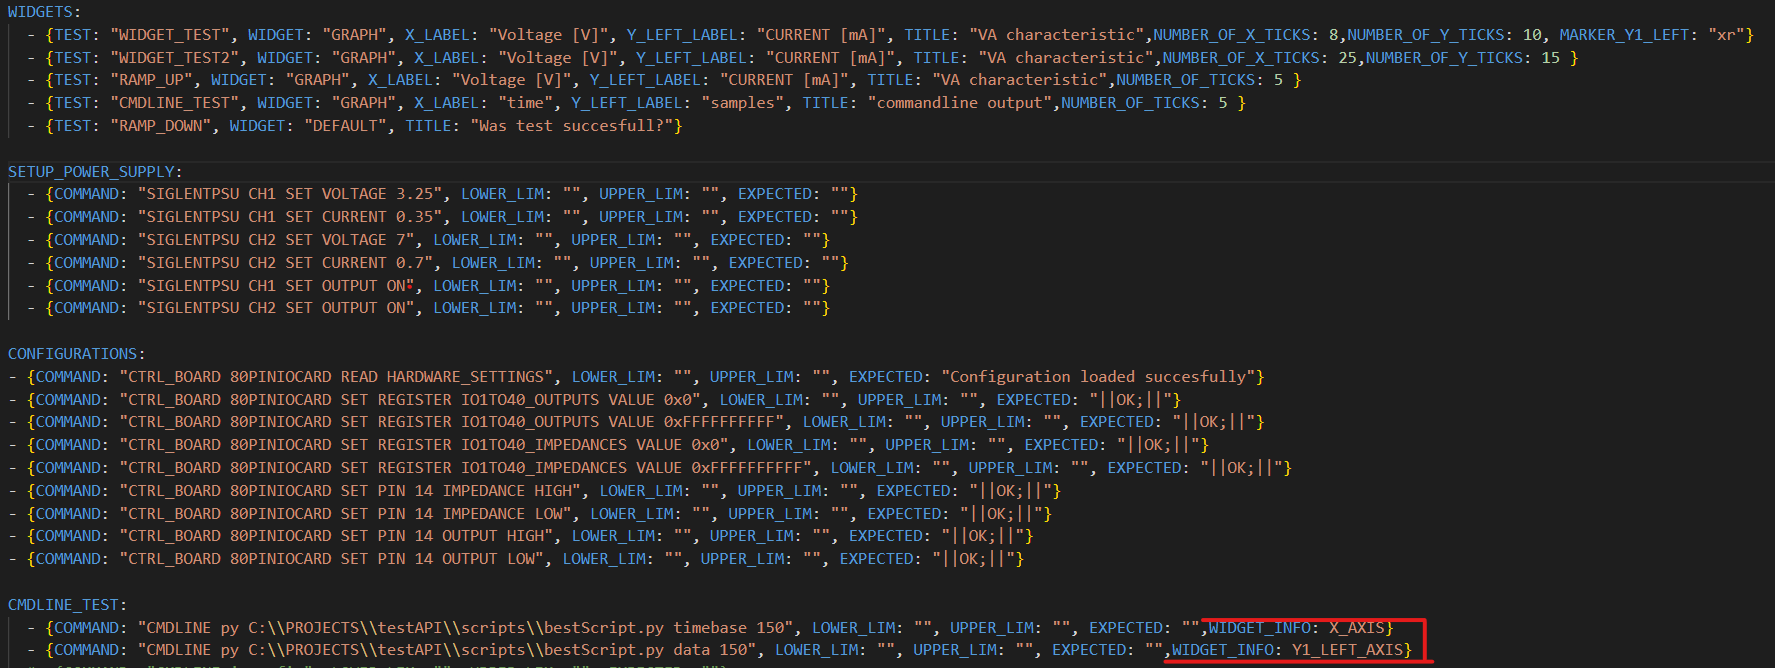
\includegraphics[width = 0.9\textwidth]{obrazky/test_result_class.png}
    \caption{PC aplikace - tests.yaml ukázka}
    \label{fig: tests yaml}
\end{figure}

Podrobný popis konfiguračního soboru test.yaml a všech jeho funkcí by byl příliš zdlouhavý.
Obecně jsou podporovány všechny příkazy, které nabízí Device Hub Vrstva.
Hlavní myšlenkou je demonstrovat, že lze pomocí tohoto souboru dynamicky definovat testy a jejich widgety (způsob zobrazení). 
To, jaký widget bude použit pro zvolený test lze měnit v části "WIDGETS" tests.yaml souboru. Například pro test "CMDLINE\_TEST" je zvolen
widget "GRAPH", což v PC aplikaci nastaví zobrazení v podobě grafu.
Následně v červeně označené části je definováno, které data budou zobrazeny na určitých osách grafu.\\

Po spuštění testu lze v PC aplikaci zobrazit výsledky v následující podobě.
\begin{figure}[ht!]
    \centering
    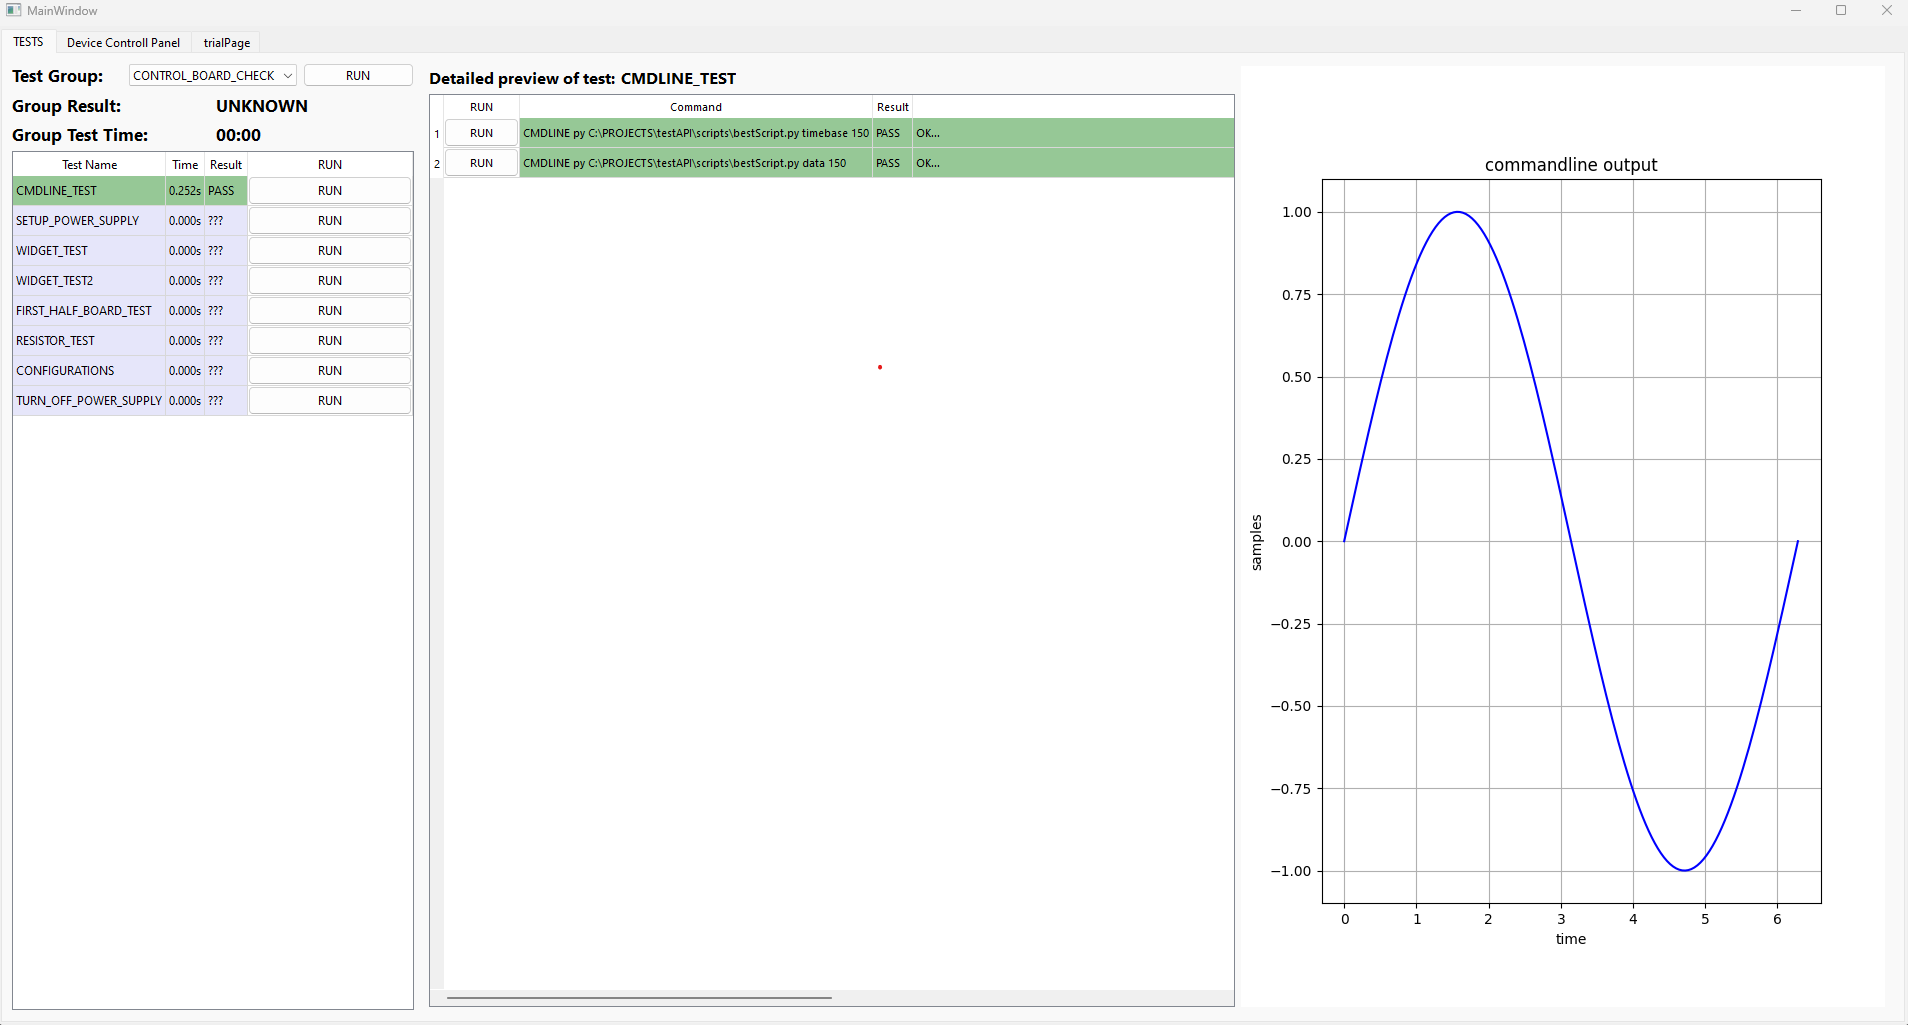
\includegraphics[width = 0.9\textwidth]{obrazky/test_result_widget_graph.png}
    \caption{PC aplikace - tests.yaml ukázka výsledku testů - graf}
    \label{fig: tests yaml graf}
\end{figure}

Pokud by byl spuštěn například test SETUP\_POWER\_SUPPLY, kterým mimojiné byl nastavován laboratorní 
zdroj SIGLENT SPD3303X-E, pomocí kterého byla deska napájena v době měření všech výsledků zobrazených v diplomové práci.
PC aplikace zobrazí v pravé části výchozí widget, protože v konfiguračním souboru nebyl pro tento test žádný widget definován.
\begin{figure}[ht!]
    \centering
    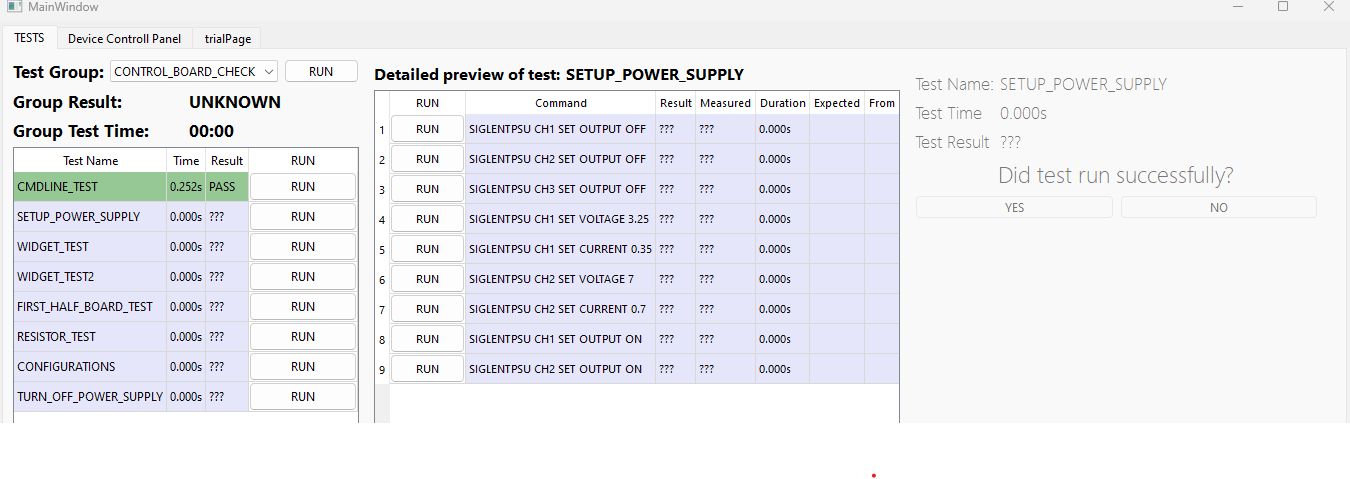
\includegraphics[width = 0.9\textwidth]{obrazky/test_result_widget_prompt.png}
    \caption{PC aplikace - tests.yaml ukázka výsledku testů - default}
    \label{fig: tests yaml default}
\end{figure}


\subsection{konfigurační soubor tests.yaml}
Dalším konfiguračním souborem, který je v diplomové práci použit je soubor hardwareConfig.yaml. Tento soubor je oproti
předchozího souboru tests.yaml nutný k úspěšné kompilaci programu. Nicméně jeho obsah je možné měnit i po kompilaci.
Následující obrázek je ukázkou výstřižku z tohoto souboru.
\begin{figure}[ht!]
    \centering
    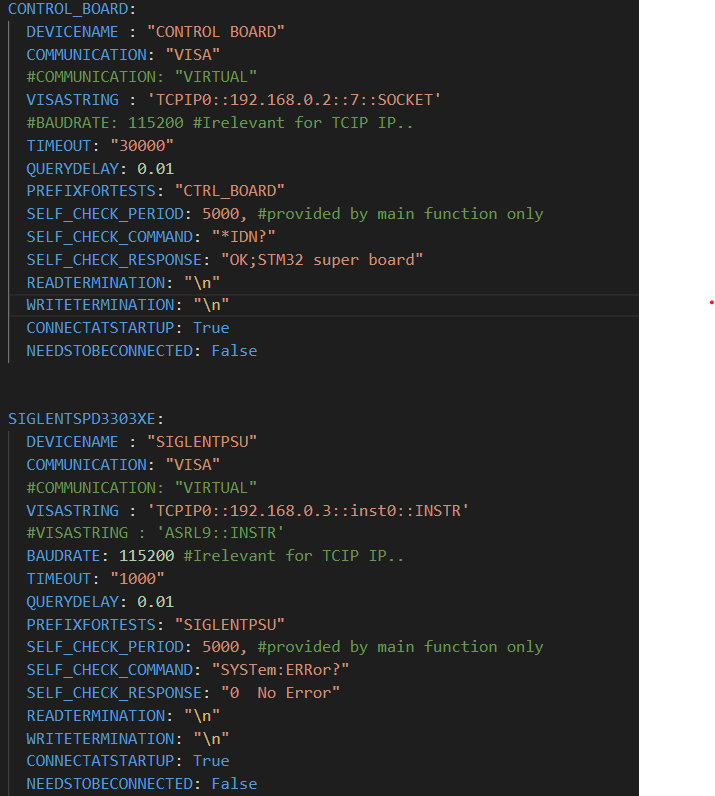
\includegraphics[width = 0.55\textwidth]{obrazky/hardwareConfig.png}
    \caption{PC aplikace - hardwareConfig.yaml}
    \label{fig: hardwareConfig yaml}
\end{figure}
\clearpage

Na výstřižku jsou zobrazeny konfigurace pro 2 zařízení, které používají pro Raw low layer právě komunikaci pomocí VISA knihoven.
Jsou zde nastaveny nejdůležitější parametry, které jsou potřebné pro komunikaci s daným zařízením. Zajímavou možností je zvolit
nastavení položky "COMMUNICATION" z VISA na VIRTUAL. Tímto lze aplikaci používat i v případě, že není k dispozici daný hardware.
Veškeré testy pro dané zařízení pak probíhají v tzv. "virtuálním módu". Pro některá zařízení je opravdu emulován virtuální hardware
a pro některá (včetně ovládacích karet z diplomové práce) jsou pouze navracovány hodnoty "VIRTUAL".\\

Důležitou položkou je parametr PREFIXFORTESTS, který určuje, jaký prefix bude použit pro testy, které jsou definovány v tests.yaml.
Například pro zmíňený test SETUP\_POWER\_SUPPLY z obrázku \ref{fig: tests yaml} je prefix "SIGLENTPSU". Každý test začínající na tento
prefix je pak přesměrován do příslušného hardwaru. V diplomové práci je využito těchto prefixů pro rozlišení jednotlivých ovládacích karet.